\documentclass{bmvc2k}
%% Enter your paper number here for the review copy
% \bmvcreviewcopy{??}

% \usepackage[brazilian]{babel}
\usepackage[utf8]{inputenc}
\usepackage{listings}

\title{Explorando o OpenCV, reconhecendo cores}

% Enter the paper's authors in order
% \addauthor{Name}{email/homepage}{INSTITUTION_CODE}
\addauthor{Víctor Rodrigues Pacheco\\Matrícula: 17/0063879}{victorrpacheco98@gmail.com}{1}

% Enter the institutions
% \addinstitution{Name\\Address}
\addinstitution{
  Departamento de Ci\^encia da Comptuta\c{c}\~ao\\
  Universidade de Bras\'{\i}lia\\
  Campus Darcy Ribeiro, Asa Norte\\
  Bras\'{\i}lia-DF, CEP 70910-900, Brazil,  
}

\runninghead{Victor Pacheco}{Princípios da visão computacional -- \today}

% Any macro definitions you would like to include
% These are not defined in the style file, because they don't begin
% with \bmva, so they might conflict with the user's own macros.
% The \bmvaOneDot macro adds a full stop unless there is one in the
% text already.
\def\eg{\emph{e.g}\bmvaOneDot}
\def\Eg{\emph{E.g}\bmvaOneDot}
\def\etal{\emph{et al}\bmvaOneDot}

%-------------------------------------------------------------------------
% Document starts here
\begin{document}

\maketitle

\begin{abstract}
Esse trbalho exalta o uso biblioteca multiplataforma OpenCV como uma ferramenta para a visão computacional quando combinada à linguagem de programação Python por meio do desenvolvimento de códigos para a idenficiaçãode posições de pixels e cores e destaque de pixels específicos visando auxiliar a entrada de entusiastas no universo da visão computacional de forma didática e open source.

\end{abstract}

%-------------------------------------------------------------------------
\section{Introduction}
\label{sec:intro}
A Biblioteca multiplataforma OpenCV \cite{[OpenCVOrg]} que teve seu desenvolvimento formentado pela intel na virada do milênio auxilia a entrada de leigos no universo da  visão computacional e traz avanço e unificação para os mais experientes.
O processo de tratamento de imagem com base em suas cores é o primeiro prjeto de muitos que buscam mais conhecimento na área, se assimilando ao "Hello World" e ao "Piscar LED".
Usuários de OpenCV podem utilizar desse artigo para a introdução ao uso da linguagem com a biblioteca. É importante ressaltar o caráter Open Source da linguagem e sua grande comunidade apta para auxiliar. 
Neste trabalho foram desenvolvidos para análise de imagens pixel a pixel e tratamento de imagem para destaque com base em cor tanto para arquivos JPG quanto para arquivos AVI. Isso visa capacitar de forma técnica para propiciar o desenvolvimento de projetos mais complexos futuramente.

\subsection{Repositório}
Os código desenvolvidos nesse projeto estão disponíveis de forma Open Source na platafora GitHub no repositório do autor disponível em \url{https://github.com/VictorRPacheco/ExplorandoOpenCV}.
Para saber mais sobre o uso da ferramenta GitHub é recomendado o tutorial de Roger Dudler \url{https://rogerdudler.github.io/git-guide/index.pt_BR.html} que introduz o básico da ferramenta

\section{Desenvolvimento}
\subsection{Sistema}
Todos os códigos foram desenvolvidos e testados em uma máquina virtual Oracle VirtualBox \cite{[VM]} com as seguintes características:
\begin{itemize}
    \item Versão VM 6.0.4
    \item Versão OS: Ubuntu 16.04 LTS 64-bits
    \item Versão Python: 2.7
    \item Versão OpenCV: 3.2.0
\end{itemize}
 A máquina virtual utilizada está disponível em \url{https://mega.nz/#F!MEgzWSiS!8HuAvnv2mFd0pyBnl2VVjg} de autoria de Mateus Berardo de Souza Terra.
 
\subsection{Requisitos}
O sistema atende quatro requisitos, especificados a seguir:

\begin{enumerate}
    \item Elabore uma aplicação utilizando OpenCV que abra um arquivo de imagem (do tipo JPG) e que permita ao usuário clicar com o botão esquerdo do mouse sobre um ponto na área da imagem e mostre no terminal a coordenada do ponto (row,column) na imagem, informando os valores do pixel RGB, quando a imagem for colorida ou o valor da intensidade do pixel quando a imagem for em nível de cinza (greyscale).
    \item  Repita o procedimento desenvolvido no Requisito 1 e crie uma rotina de seleção de pixels baseado na cor de onde for clicado. Seu programa deve comparar o valor da cor (ou tom de cinza) de todos os pixels da imagem com o valor da cor (ou tom de cinza) de onde foi clicado. Se a diferença entre esses valores for menor que 13, marque o pixel com a cor vermelha e exiba o resultado na tela.
    \item  Repita o procedimento desenvolvido no Requisito 2, em que ao invés de abrir uma imagem, abra um arquivo de vídeo (padrão avi ou x264) e realize os mesmos procedimentos do Requisito 2 durante toda a execução do vídeo. Cada vez que o usuário clica na imagem, o valor de referência deve ser atualizado.
    \item Repita o procedimento desenvolvido no Requisito 3, em que ao invés de abrir um arquivo de vídeo, a aplicação abra o streaming de vídeo de uma webcam ou câmera USB conectada ao computador e realize todos os procedimentos solicitados no requisito 3.
\end{enumerate}

\subsection{Funcionamento}
Para o funcionamento do código é necessário possuir OpenCV versão 3 compativel instalado em sua máquina, além de Python 2.
Para executar o código basta entrar na parta /src e executar o comando:
\begin{lstlisting}
python Trabalho1.py
\end{lstlisting}
Logo o programa indaga o usuário sobre qual função ele deve executar conforme os requisitos descritos. Dependendo da opção escolhida ele pede uma entrada de imagem ou vídeo para a correta execução ou que opte por um dos arquivos padrão de teste.
Com o arquivo aberto ele chamada a função Cor\_e\_Posicao resposável por identificar a posição e cor do pixel selecionado pelo usuário utilizando o cursor do mouse e logo em seguinda mostra o resultado no terminal.

\begin{lstlisting}
def Cor\_e\_Posicao(event, x, y, flags, param):\n
  global clickPoint
  global color

  if event == cv2.EVENT_LBUTTONDOWN:
    clickPoint = [x, y]
    color = image[y,x]
    print("----------------------")		
    #Identidica se a imagem eh em tons de cinza
    if color[0] == color[1] == color[2]:
      print"Posicao [X, Y]: ", (x, y), "Intensidade: ",
color[0]
    else:
      print "Posicao [X, Y]: ", (x, y), "Cor: ", str(color)
\end{lstlisting}

Para o destaque em arquivos Preto e branco foi utilizado como critério a intensidade do pixel, variando de 0 a 255 destacando os que satisfazem a equação \ref{eq:variacaoP}:

\begin{equation}
\label{eq:variacaoP}	|p{1}-p{0}| < 13
\end{equation}

Onde ($p{0}$) é o valor de um pixel indicado pelo usuário com o auxilio do cursor do mouse e ($p{1}$) representa o valor do pixel analisado para destaque.

Para arquivos coloridos que apresentam cores em 3 camadas é utilizada a diferença euclidiana \cite{[DistanciaEuclidiana]} para selecionar os pixels que devem ser destacados satisfazendo a equação \ref{eq:euclidiano} e \ref{eq:euclidProximo}:

\begin{equation}
\label{eq:euclidiano}	
\Delta{euclidiano}=\sqrt{ |R{1}-R{0}|^2+|G{1}-G{0}|^2+|B{1}-B{0}|^2}
\end{equation}

\begin{equation}
\label{eq:euclidProximo}	\Delta{euclidiano} < 13
\end{equation}

Onde o valor de ($\Delta{euclidiano}$) da \ref{eq:euclidiano} é calculado com base nos valores ($R{1}$), ($G{1}$) e ($B{1}$) que representam a cor do pixel que está sendo analizado e ($R{0}$),($G{0}$) e ($B{0}$) provenientes de um pixel indicado pelo usuário.
Logo em seguida esse valor é utilizado em uma comparação com segundo a equação \ref{eq:euclidProximo} para gerar um valor booleano indicando True para pixels que devem ser destacados.
O destaque ocorre utilizando a biblioteca NumPy \cite{[NumPy]} para otimizar o uso das matrizes.

\section{Resultados}
Utilizando como base o tutorial \cite{[PyImageSearch]} para criação da função de identificação de cor e posição dos pixels selecionados pelo usuário permetiu a imprimir no terminal os dados do pixel selecionado. No momento de criação da matriz contendo os pixels que devem ser destacados seguindo as equações \ref{eq:euclidiano} e \ref{eq:euclidProximo} se obteve uma boa perfomace para imagens, porém ao se utilizar uma máquina virtual com recursos limitados há quedas de frames para vídeos de resoluções elevadas no momento de destaque de cores similares.
O uso da camera trouxe bons resultados, sendo utilizado o tutorial \cite{[CameraTest]}, funcionou quase que em tempo real com quantidade constante de fraimes.

\begin{figure}[h!]
\begin{tabular}{ccc}
	\bmvaHangBox{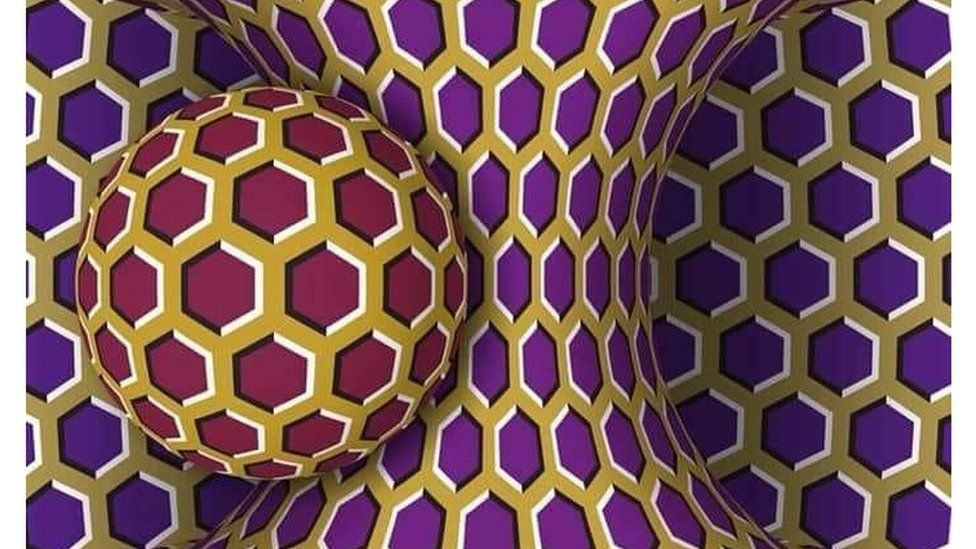
\includegraphics[height=3.5cm]{Figs/test.jpg}}&
	\bmvaHangBox{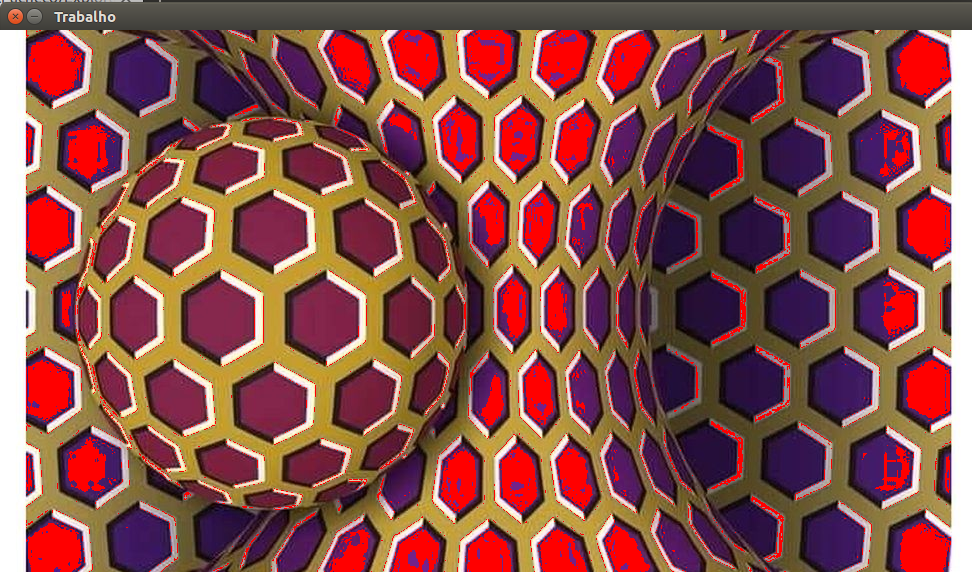
\includegraphics[height=3.5cm]{Figs/test1.png}}\\\\
	(a)&(b)
\end{tabular}
\caption{(a) Imagem de entrada do requisito2; (b) Saída após o usuário ter clicado em um ponto no requisito2.}
\begin{tabular}{ccc}
	\bmvaHangBox{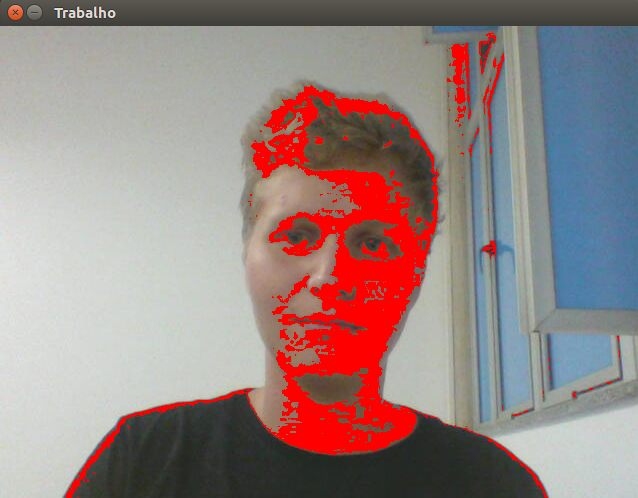
\includegraphics[height=3.5cm]{Figs/Test2.png}}&
	\bmvaHangBox{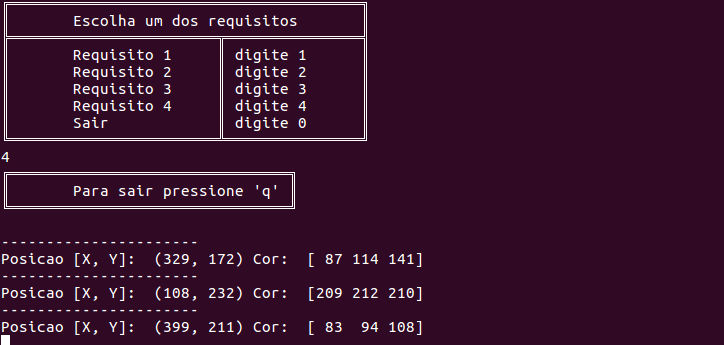
\includegraphics[height=3.5cm]{Figs/Test2Terminal.png}}\\\\
	(c)&(d)
\end{tabular}

\caption{(c) Saída do requisito 4 após clique do usuário; (d) Saída no terminal com as coordenadas e cor do ponto do requisito 4.}
	\label{fig:terminal}
\end{figure}

\section{Conclusão}
Pode-se concluir que o trabalho foi bem sucedido pois foi possível cumprir todos os requisitos de maneira eficiente utilizando a biblioteca OpenCV alinhada com a linguagem Python.
Outro ponto a ser ressaltado é o desenvolvimento técnico que foi alcançado permitindo o desenvolvimento de futuros projetos envolvendo  a biblioteca OpenCV para visão computacional de forma mais intuitiva.
%-------------------------------------------------------------------------
\bibliography{refs}
\end{document}
